\chapter{Experiments and Evaluation}
In this chapter, I present the implementation details of the two state-of-the-art models, 
along with the experiments' results and evaluation. Due to the significant training time 
of these state-of-the-art models and the limited computing resources(one free GPU from Colab), 
I decided to use one simpler dataset \cite{valada16iser} instead of the benchmark datasets 
for my project. In addition, most of the experiments were conducted in Pix2pixHD because 
the only difference for Pix2pixHD and SPADE is the generator, it is not necessary to carry 
out the experiments again on SPADE again.

\section{Dataset}
During the training of Pix2pixHD model, I experimented several different datasets, including 
benchmark datasets such as ADE20K\cite{zhou2017scene} and Cityscapes\cite{Cordts2016Cityscapes}, 
the simpler and smaller freiburg forest dataset \cite{valada16iser}. In my perspective, the 
freiburg forest dataset \cite{valada16iser} is more suitable for my project.
\subsection{Benchmark Datasets}
For image translation tasks, the training data we need are pairs of segmentation map and 
photorealistic images, which is exactly the same training data used for image segmentation 
tasks. Therefore, there are several popular benchmark datasets containing this kind of data, 
including coco-stuff\cite{caesar2018cvpr}, ADE20K\cite{zhou2017scene}, 
Cityscapes\cite{Cordts2016Cityscapes} which contain numerous 
classes of objects(e.g. Cityscapes have 30 classes of objects).
I have tried ADE20K and Cityscapes in the early stage of experiments:
\begin{itemize}
    \item ADE20K is a fully annotated image dataset designed for semantic segmentation, 
    there are 20210, 2000, 3000 images in the training, validation, testing set. All the 
    images in the training and validation set are annotated with objects with different 
    colors, many of them even get annotated with their parts. Unlike Cityscapes where 
    all the images are the scenes of cities, ADE20K covers various scenarios including 
    airfields, airports, houses, hospitals, etc. which makes the model even more 
    difficult to learn how to generate all these objects for they do not appear in the 
    similar environments. The dataset is around 4GB.
    \item Cityscapes dataset is a dataset focuses on semantic understanding of urban street 
    scenes including scenes from 50 cities, all seasons except winter, different 
    weather conditions, with 30 classes of objects. There are 5000 fine annotated 
    images for us to use. The real images are in high resolution so it is around 11GB
    large in total, also a large number of classes has also increased the difficulties 
    for our model to generate decent photorealistic images. 
\end{itemize}
If we want to achieve decent results on the testing set, we will 
have to train on all the images provided in the training set so that our model can adapt 
to different scenarios and learn the patterns of different kinds of objects. Nevertheless, 
even the smallest dataset among them has more than 4GB data, which makes each experiment 
pf training lasts for days on the free GPU that Colab provides. This is the reason why 
in the experiment, I only use a small part of those data and keep the training time 
within an acceptable amount of time. 
\subsection{Freiburg Forest Dataset}
\label{sec:freiburg}
Freiburg Forest dataset was collected using an autonomous mobile robot equipped with 
cameras, where all scenes were recorded at 20HZ with $1024\times768$ resolution. The 
annotated images containing only 5 classes of objects including object, trail, grass, sky 
and vegetation, 230 pairs of images(each pair consists of a segmentation
map and a real photo) in the training set and 136 pairs of images in the testing set. 
The small scale of such dataset increases the fault tolerance for each training, i.e. I do 
not have to wait for hours to see the wrong intermediate results and start all over. 
Because the scenes are all similar and the objects are simple, so it does not need to train
on considerable training data to generate decent and clear images like the benchmark datasets,
which compensates the limited computing resources issue.
Even if this is a comparable small dataset, it still takes hours to train one single model. 
For downloading the annotated dataset(around 1GB) and more details, please 
check \href{http://deepscene.cs.uni-freiburg.de}{DeepScene} website.
\subsection{Preprocessing}
Pytorch allows us to load images from folders dynamically with “CustomDataset” function, so 
what I have to do is use “glob” function to find the pair of segmentation map and real photo 
image, and then use PIL library to corp the image into the required resolution(e.g. $512\times256$), 
and then return them to Pytorch.

Data augmentation techniques such as rotation or flipping can be applied, however, 
I do not see obvious improvement when I run the tutorial script of Pix2pix model, 
this is why I do not apply any of those to my implementation.

\section{Pix2pixHD Implementation}
The implementation of my Pix2pixHD basically follows the architecture from the paper, 
except I only uses 6 residual blocks instead of 9, you can see the architecture of the 
generator in figure \ref{fig:pix2pix-generator} and table \ref{Pix2pixHD generator table},  
the discriminator architecture in table \ref{Pix2pixHD discriminator table}. The final
solution is to train the networks with VGG loss on the Freiburg dataset. Before that, 
I ran simulations on a small portion ADE20K to determine if the VGG loss component is 
effective or not. I also ran simulations on the Cityscapes dataset and tries to achieve similar 
results as the paper, but they all have some problems. 

Adam optimizer is used for training.
In terms of the learning rates, I set a higher learning rate for the generator instead of using 
identical learning rate because I noticed the discriminator loss can get down to a low value 
after just a few epochs of training while the generator merely reduce its loss a little 
each epoch, therefore, I hope I can speed up the training of the generator while keeping the 
discriminator as before. The generator learning rate $2\times10^{-5}$ and discriminator learning 
rate $10^{-5}$ seems to work fine for me. 

The whole GAN model training is a cyclic process, where for each epoch:
\begin{enumerate}
    \item Get a pair of images from the training dataset
    \item Generator generates a fake image according to input segmentation map
    \item Calculate generator loss(GAN loss, feature matching loss and VGG perceptual loss)
    \item Calculate discriminator loss(real loss, fake loss)
    \item Update weights of the models by backward pass
\end{enumerate}

\subsection{VGG Loss Experiment}
Even though in the paper the author claims that VGG loss does not have a significant influence on 
the generated image, I found the opposite conclusion when training the Pix2pixHD model on ADE20K 
dataset. In order to reduce the training time, I only uses air base images from ADE20K. 

At first, 
I did not use VGG loss component, the generator can learn to generate the shape of the objects 
however it cannot learn how to fill in the colors. As you can see in figure \ref{fig:without-VGG}, 
the generator can only learn the shape of the plane and people, but the generated picture 
consists of only two color mosaics.
\begin{figure}[H]
    \begin{center}
    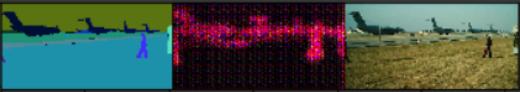
\includegraphics[width=10cm]{figures/without-VGG}
    \end{center}
    \caption{Example generated image without VGG loss during training}
    \label{fig:without-VGG}
\end{figure}

On the other hand, after adding the VGG loss component, the generator returns to normal, as you 
can see in figure \ref{fig:with-VGG}. All simulations after this used VGG loss as well.
\begin{figure}[H]
    \begin{center}
    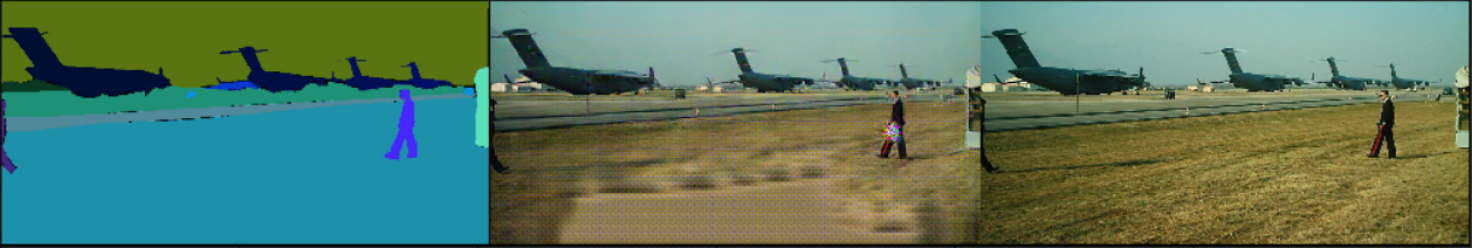
\includegraphics[width=10cm]{figures/with-VGG}
    \end{center}
    \caption{Example generated image with VGG loss during training}
    \label{fig:with-VGG}
\end{figure}

The VGG perceptual loss we use here is based on VGG-19\cite{articleVGG}, which is a very powerful
neural network trained for image classification. Using VGG loss means we compare the differences 
between the features extracted from the real images by a pre-trained VGG network and the features from 
the generator, since VGG network is very powerful, if our generator generates similar features as 
those from VGG, the final output should be excellent as well. The VGG perceptual loss has achieved 
marvelous results \cite{DBLP:journals/corr/JohnsonAL16} in style transfer tasks.     

Even with the help of VGG loss, merely using a few categories of images in ADE20K cannot achieve 
decent results when it comes to testing phases. As you can see in figure \ref{fig:ADE20K-test}, 
the model seemed to suffer from overfitting issue, i.e. the model performs quite well on 
a training set, but perform poorly at testing phases. This may because the training data is not 
enough, for example, during the training phase, the generator never encounter enough patterns of 
a person in front of the camera, so it does not know what pattern it should fill into that 
shape, that is why we can only see mosaics. Next, I experimented with several cities images 
from the Cityscapes dataset.
\begin{figure}[H]
    \begin{center}
    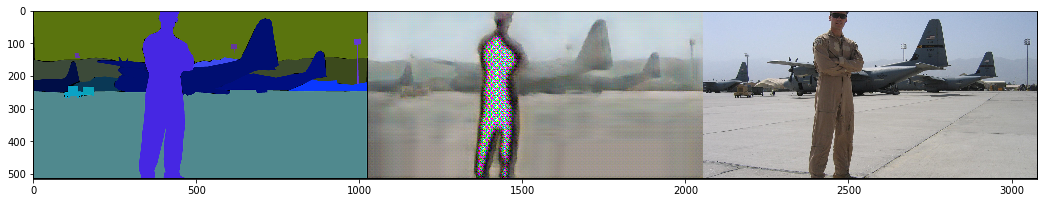
\includegraphics[width=10cm]{figures/ade20k-test}
    \end{center}
    \caption{Example generated image during testing phase with ADE20K air base images}
    \label{fig:ADE20K-test}
\end{figure}

\subsection{Cityscapes Experiment}
I spent a lot of time running simulation on Cityscapes dataset, despite I used only 3000 
pairs of images out of 5000. For the local enhancer, it took about 500 seconds for one 
epoch. The following figures \ref{fig:Cityscapes-train} \ref{fig:Cityscapes-test} are my 
results after 500 epochs of training on the global generator and 200 epochs of training 
on local enhancer, we can still observe the overfitting kind of issue as the training 
results look very realistic while the testing results have blur patterns everywhere 
which does not sound real to me.
\begin{figure}[H]
    \begin{center}
    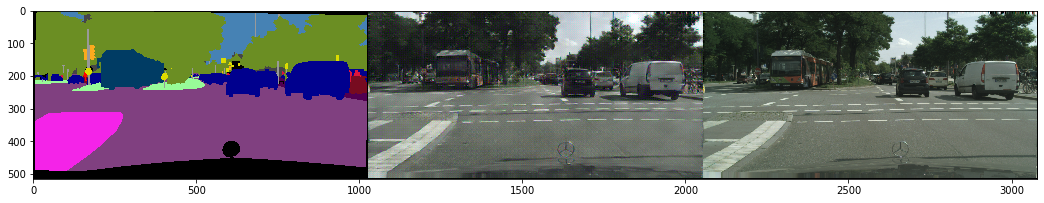
\includegraphics[width=14cm]{figures/cityscapes-train}
    \end{center}
    \caption{Example generated image during training phase with part of Cityscapes}
    \label{fig:Cityscapes-train}
\end{figure}

\begin{figure}[H]
    \begin{center}
    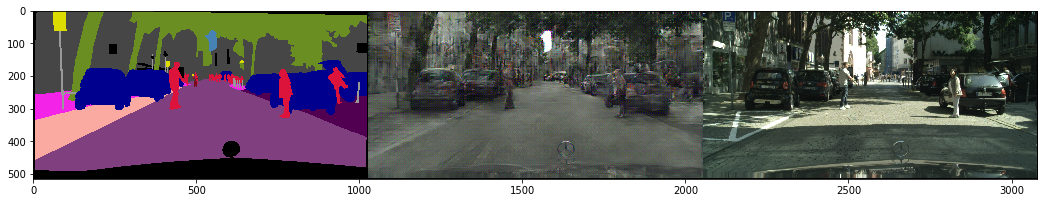
\includegraphics[width=14cm]{figures/cityscapes-test}
    \end{center}
    \caption{Example generated image during testing phase with part of Cityscapes}
    \label{fig:Cityscapes-test}
\end{figure}

In my opinion, training for more epochs or adjust the hyperparameters are not likely to fix 
this issue since the training results have already been good enough, so it is more like a 
overfitting issue than an underfitting issue to me. Increasing the amount of images used for 
training is very likely to help, however, the significant training time makes it too 
difficult to finish on Colab. The reason for all these is that Cityscapes dataset contains 
too many classes of objects, and some class of objects have complex textures, which requires 
our model to learn from more training image if we want to generate them correctly without too 
many blurs.
This is why I decided to use a Cityscapes like dataset with 
fewer classes of objects and simpler textures for each class of objects, and the freiburg 
forest dataset just meets all the requirements.
\subsection{Train on Freiburg Forest Dataset}
We have already introduced freiburg forest dataset in \ref{sec:freiburg}. I trained the 
global generator for 200 epochs first, the training remain stable even we increase the 
learning rate for the generator which seems to be a success. I tracked the loss of the 
generator and discriminator for each epoch and figure \ref{fig:global-generator-loss} is the 
curve chart of the loss values for global generator and discriminator, which looks 
making sense. 
\begin{figure}[H]
    \begin{center}
    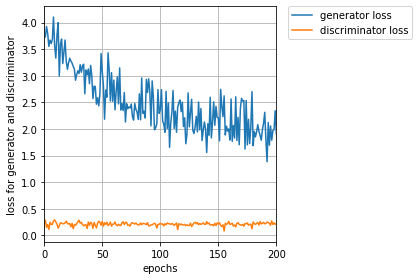
\includegraphics[width=8cm]{figures/global-generator-loss}
    \end{center}
    \caption{Loss values curve of global generator and discriminator during training}
    \label{fig:global-generator-loss}
\end{figure}
The global generator can generate decent images even when at testing phase, however,
we do observe many “dots” around the generated image as figure \ref{fig:global-generator-output}, 
this can be alleviated after 
we trained for certain epochs for the local enhancer.
\begin{figure}[H]
    \begin{center}
    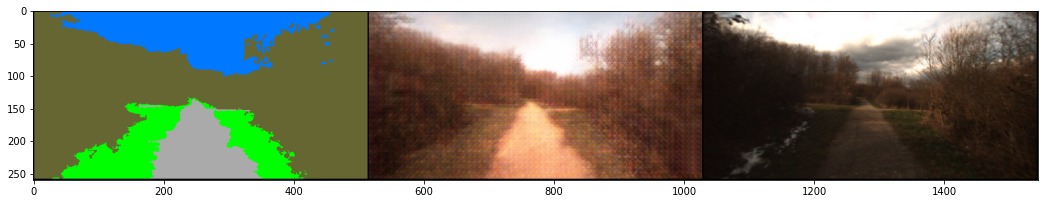
\includegraphics[width=14cm]{figures/global-generator-output}
    \end{center}
    \caption{Example output from Pix2pixHD global generator during testing}
    \label{fig:global-generator-output}
\end{figure}

I trained 100 epochs(about 4-5 hours) for local enhancer and it can already produce 
high quality images as figure \ref{fig:local-enhancer-output}. 
Since local enhancer aims to generate high resolution images, it alleviates the 
“dots” problem mentioned in global generator significantly.
Even you may still observe some blurs in certain areas, the overall quality is 
acceptable given the computing resources and training time we spent.
All the training parameters remain unchanged, and the training is also very stable, 
as you can see from figure \ref{fig:local-enhancer-loss}.
\begin{figure}[H]
    \begin{center}
    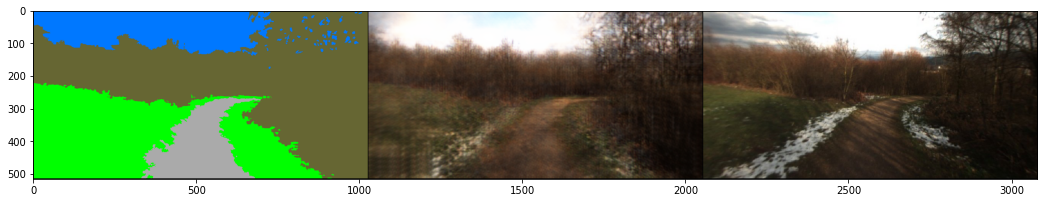
\includegraphics[width=14cm]{figures/local-enhancer-output}
    \end{center}
    \caption{Example output from Pix2pixHD local enhancer during testing}
    \label{fig:local-enhancer-output}
\end{figure}

\begin{figure}[H]
    \begin{center}
    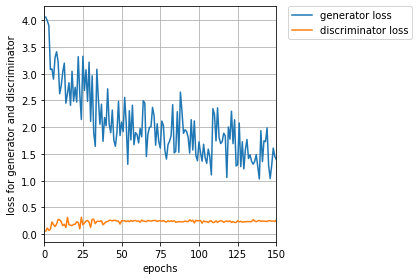
\includegraphics[width=8cm]{figures/local-enhancer-loss}
    \end{center}
    \caption{Loss values curve of local enhancer and discriminator during training}
    \label{fig:local-enhancer-loss}
\end{figure}

\section{SPADE Implementation}
\nocite{SPADE-blog-1}
\nocite{SPADE-blog-2}
SPADE is proposed after Pix2pixHD, which is trying to improve the results of Pix2pixHD further. 
The paper of SPADE provided the implementation of the networks in detail, so it is not a very 
difficult task to build the generator, also, apart from the generator, we can using the same 
code as Pix2pixHD implementation since they follow the same structure of GAN training.
\subsection{Generator of SPADE}
The generator of SPADE can be directly built according to the “Additional Implementation Details”
in the paper \cite{park2019SPADE} by stacking the building blocks. The order of building such 
network is to build the SPADE block first, and then use SPADE blocks to build SPADE residual 
blocks, and in the end we can integrate SPADE residual blocks with the traditional GAN generator 
structure to build the SPADE generator. Note we use $512\times256$ resolution images, 
instead of $256\times256$ in the original paper, so we need 
to make small changes in terms of the tensor shapes, you can check the final network structure 
with table \ref{SPADE generator table}. 
\begin{figure}[H]
    \begin{center}
    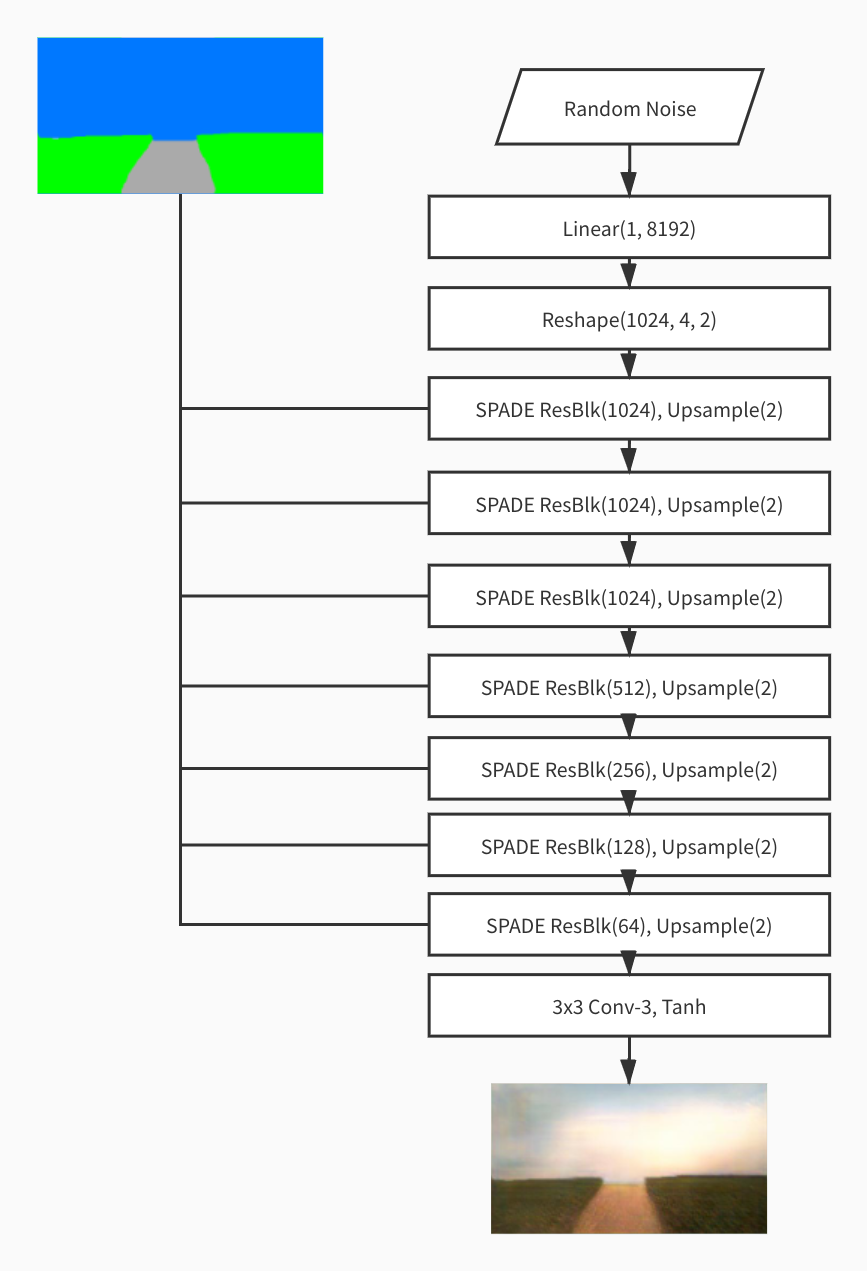
\includegraphics[width=8cm]{figures/SPADE-imp-generator}
    \end{center}
    \caption{SPADE Generator for Freiburg Forest Dataset}
    \label{fig:SPADE-imp-generator}
\end{figure} 

As shown in figure \ref{fig:SPADE-imp-generator}, the generation process is like we first 
generate random input noises shaped (1, 8192) for the batch size we use is one, we then 
reshape 8192 into (1024, 4, 2), next, the input noises will go through seven SPADE residual blocks 
together with the segmentation map, the output tensor will be upsampled 
by 2 after each SPADE residual block, eventually, a convolution layer with tanh activation 
will convert the tensor into images. You can refer to the SPADE block and SPADE residual block 
structure that the generator depends on in figure \ref{fig:SPADE-Block} and 
figure \ref{fig:SPADE-ResBlock} in chapter 2.
\subsection{Training}
The training configuration remained the same as Pix2pixHD, the only significant difference between 
these two model is the generator. I trained the SPADE model for 150 epochs and it can produce 
clear photorealistic images as figure \ref{fig:SPADE-output}. The loss value curve of 
the SPADE model training is also stable, the loss of the generator went down gradually as shown 
in figure \ref{fig:SPADE-loss}. 
\begin{figure}[H]
    \begin{center}
    \includegraphics[width=14cm]{figures/SPADE-output}
    \end{center}
    \caption{Example output from SPADE generator during testing}
    \label{fig:SPADE-output}
\end{figure}
\begin{figure}[H]
    \begin{center}
    \includegraphics[width=8cm]{figures/SPADE-loss}
    \end{center}
    \caption{Loss values curve of SPADE generator during training}
    \label{fig:SPADE-loss}
\end{figure}
\section{Comparison}
If we compare the results of the Pix2pixHD model(figure \ref{fig:local-enhancer-output}) and 
SPADE model(figure \ref{fig:SPADE-output}), we might find SPADE model has the following 
advantages over Pix2pixHD: 
\begin{itemize}
    \item Clearer images without any “dot”: although the generated images are not perfectly 
    clear without any blur, it does remove the “dots” observed in the output of Pix2pixHD 
    model. We need more training data and more training time if we want to learn the textures 
    better of each class of objects.
    \item Only need to train one generator: when doing the implementation, I found training 
    two generator for Pix2pixHD model really annoying, two generators' training require more 
    overall training time than one more complex model.
    \item Possibility of applying style transfer: since in the SPADE model, we no longer uses 
    conditional GAN structure for the genenrator, we remove the encoder part of the conditional 
    GAN generator, which adds the possibility of building another encoder that can encode a 
    style image and achieve style transfer effects. I have not implemented this feature which I 
    discuss further in section \ref{sec:future work}.
\end{itemize}

Nevertheless, I think Pix2pixHD is still the state-of-the-art model because it offers a way for 
us to generate high-resolution images. The SPADE model can be used for higher resolution image 
translation in theory, but it has already needed a lot of training time, generating high-resolution 
images will require even more training time.